\documentclass[11pt]{scrartcl}
\usepackage{ucs}
\usepackage{float}
\usepackage[utf8x]{inputenc}
\usepackage{ngerman}
\usepackage{amsmath,amssymb,amstext}
\usepackage{graphicx}
\usepackage{tabularx}
\usepackage[square]{natbib}
\usepackage[justification=RaggedRight, singlelinecheck=false]{caption} 
\usepackage{fancyhdr}

\pagestyle{fancy}
\lfoot{Adin Karic}
\rfoot{\today{}}

\title{Sicherheit}
\author{Adin Karic}
\date{\today{}}

\begin{document}

\maketitle
\pagebreak
\tableofcontents
\pagebreak

\section{Grundlagen Security}
\label{sec:basics-security-process}
% Moderne Kryptographie 2

\subsection{Sicherheitsziele}
\label{sec:security goals}
Im Allgemeinen kann man die vier folgenden wichtigen Schutzziele definiere\cite{1}:\\
\begin{itemize}
\item Vertraulichkeit – Schutz vor unautorisiertem Zugang zu Informationen.
\item Integrität - Schutz vor unautorisierter unbemerkter Änderung von Informationen.
\item Verfügbarkeit - Schutz vor unautorisiertem Beschlagnehmen von Informationen oder Ressourcen.
\item Zurechenbarkeit – für Aktionen und Ereignisse Verantwortliche müssen ermittelbar sein.
\end{itemize}

Für spezielle Dienste existieren verschiedene Implementierungen dieser
Schutz- oder Sicherheitsziele. Das Ziel der IT-Sicherheit ist die Gewährleistung eines Schutzlevels ausgehend von diesen Schutzzielen trotz  immer intelligenter vorgehenden Angreifern.
Verwundbarkeiten von IT-Systemen werden als Schwächen
der Systeme verstanden, die ausgenutzt werden können, um IT-Sicherheitsverletzungen
durchzuführen. Bedrohungen sind dann das Ergebnis der Ausnutzung einer oder mehrerer Verwundbarkeiten. Konkrete Anleitungen, Prozeduren oder Programme zum gezielten Ausnutzen dieser Verwundbarkeiten im System werden  Exploits genannt.\\
Um einen richtigen und sinnvollen Umgang mit Zugriffen auf IT-Ressourcen zu ermöglichen ist eine Sicherheitspolitik nötig, die eine Menge von Regeln enthält, die festlegen was erlaubt ist und was nicht. Als Sicherheitsverletzung, Attacke oder Einbruch(Intrusion) wird ein Ereignis verstanden, welches den Regeln Sicherheitspolitik zuwiderläuft.\\
Bisher wurden zum Schutz von IT-Systemen hauptsächlich präventive Verfahren (IPS) benutzt. Der massive Zuwachs an Sicherheitsvorfällen macht jedoch klar, dass präventive Maßnahmen allein nur ein gewisses Maß an Schutz bieten können.
Trotz der verstärkten Anwendung von präventiven Verfahren wurde in den letzten Jahren ein jährlicher Anstieg der beim CERT/CC (Computer Emergence Response
Team / Coordination Center) gemeldeten Vorfälle vermerkt. Ein präventiver Mechanismus kann keinen Schutz vor Missbrauchsaktionen von autorisierten Nutzern bieten \cite{2}. Daher muss man präventive Verfahren durch sogenannte reaktive Verfahren ergänzen.\\
\begin{figure}
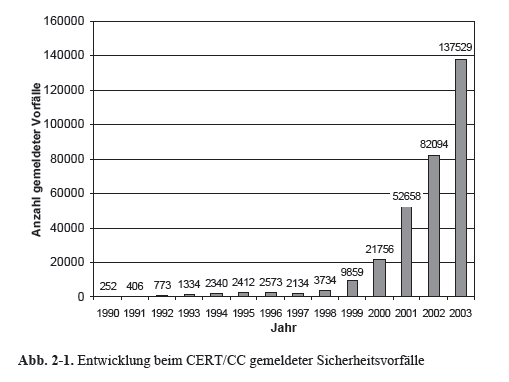
\includegraphics[width=0.45\textwidth]{aa2.png}
	\caption{Entwicklung beim CERT/CC gemeldeter Sicherheitsvorfälle \cite{5}}
	\label{fig1}
\end{figure} \noindent

Das Ziel reaktiver Maßnahmen ist also die Begrenzung und Beseitigung von verursachten Schäden sowie die schnellstmögliche Identifikation der verantwortlichen Angreifer. Nur so können die Angreifer zur Rechenschaft gezogen werden und Schadenersatzansprüchen können geltend gemacht werden. Ein positiver Nebeneffekt sind dabei die Abschreckungseffekte die entstehen und zusätzlich präventiv wirken können. \cite{2}. Die Voraussetzung für ein solches System ist eine zuverlässige Erkennung von Sicherheitsverletzungen. Hierzu werden Intrusion Detection Systeme (IDS) verwendet.\cite{3}\cite{4}\cite{5}

\section{Intrusion Detection Systeme}
\label{sec:IDS}

\subsection{Gründe für die Nutzung eines IDS}
\label{sec:reasons IDS}
Die Gründe für die Implementierung eines Intrusion Detection Systems liegen auf der Hand. Wie oben geschildert stieg die Anzahl der Angriffe bzw. Sicherheitsverletzungen in den letzten Jahren rapide an. Dieser Tendenz konnte mit der Benutzung von Intrusion Prevention Systemen (IPS- also Einbruchverhinderungssystemen) nicht entgegengesetzt werden. 
Die Bedrohungen können oftmals sehr vielfältig sein. "Der Angreifer kann zum Beispiel über Fehler in der Implementierung des  TCP/IP-Stacks Zugriff auf das System oder dessen Ressourcen erhalten. Ein Profi findet anhand einer Untersuchung des TCP/IP-Fingerprints ( nmap heraus, um welches System es sich handelt, kann durch diese Information ganz gezielt Schwachstellen suchen und nutzt diese letztendlich für einen Angriff aus."
Ohne ein Intrusion Detection System hat man keine Möglichkeit herauszufinden wie lange ein Eindringling unbemerkt blieb, wie und wann er seinen Angriff ausführte oder welcher Schaden dadurch entstand.
Die Hauptziele eines IDS sind also:\\
\begin{itemize}
\item Benachrichtigung des Admins/Sicherheitsbeauftragten im Falle eines Angriffs oder das Ergreifen von aktiven Gegenmaßnahmen
\item eine juristische Verwertbarkeit der gesammelten Daten (den Angriff betreffend)
\item die Erkennung von Verlusten(Daten z.B.)
\item der Schutz vor zukünftigen Angriffen durch die Auswertung der gesammelten Daten bei einem (simulierten) Angriff. \cite{6}
\end{itemize}

\subsection{Funktionsweise eines IDS}
\label{sec:function IDS}
Wie oben schon erwähnt ist das Ziel des Einsatzes von Intrusion-Detection-Systemen ist eine  frühzeitige Erkennung von Attacken, um den möglichen Schaden zu minimieren und
Angreifer identifizieren zu können. 

Darüber hinaus sammeln IDS Informationen über neue Angriffsmethoden welche zur Verbesserung präventiver Maßnahmen genutzt werden können. Hierzu analysiert ein IDS die Daten über Abläufe sowie Zustände von IT-Systemen. Die Defense Advanced Research Projects Agency (DARPA) initiierte ein Projekt, zur Standardisierung des Aufbaus eines IDS. Hierdurch sollte die Wiederverwendbarkeit von IDS-Komponenten erreicht werden. Das Ergebnis des Standardisierungsprozesses ist das Common Intrusion Detection Framework (CIDF) \cite{7} welches unter anderem mögliche Architekturen von Intrusion Detection Systemen beschreibt. 
Das CIDF definiert vier Arten von IDS-Komponenten:\\
\begin{itemize}
\item Ereigniskomponenten stellen die Informationen über das zu schützende IT-System
bereit. Systemfunktionen die zur Protokollierung sicherheitsrelevanter
Aktivitäten dienen sind Beispiele für Ereigniskomponenten.

\item Analysekomponenten sind für die eigentliche Erkennung von Angriffen zuständig.
Dazu analysieren sie die von den Ereigniskomponenten bereitgestellten
Informationen.

\item Datenbankkomponenten speichern weitere zur Analyse erforderliche Informationen
sowie Zwischenergebnisse.

\item Reaktionskomponenten führen auf Veranlassung durch andere IDS-Komponenten
Gegenmaßnahmen durch.
\end{itemize}

\begin{figure}
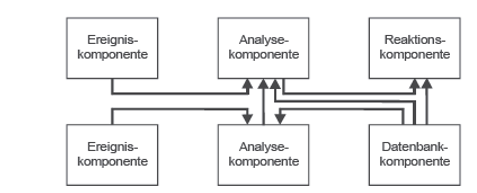
\includegraphics[width=0.45\textwidth]{aa3.png}
	\caption{Informationsaustausch verschiedener CIDF-Komponenten \cite{5}}
	\label{fig2}
\end{figure} \noindent
\subsubsection{Ereigniskomponenten und Audit}
\label{sec:ereignis und audit}

Die Voraussetzung für eine automatische Erkennung von Sicherheitsverletzungen
ist eine detaillierte Aufzeichnung von Informationen über sicherheitsrelevante Abläufe
oder Zustände des zu schützenden Systems. Hierzu wird in der Literatur oftmals der Begriff Audit verwendet.\\
Unter diesem Begriff werden Verfahren
\begin{itemize}
\item zur Protokollierung,
\item zur Analyse oder
\item zur Protokollierung und Analyse
\end{itemize}
zusammengefasst.
\subsubsection{Analyse- und Datenbankkomponenten}
\label{sec:analyse und db}
Für die eigentliche Erkennung von Sicherheitsverletzungen sind die Analysekomponenten zuständig. Je nach verwendeter Analysemethode werden dazu zusätzliche
Informationen verwendet, welche sich in den Datenbankkomponenten befinden.

Mittels entsprechender Mechanismen werden die in den Audit-
Daten protokollierten Beobachtungen analysiert, um den Zustand des
überwachten IT-Systems als sicherheitskonform oder sicherheitsverletzend zu
klassifizieren. Hierbei sind vier Werte essentiell für die Bewertung dieser Klassifikationen:\\
\begin{itemize}
\item Wahr-Positive: Beobachtungen, welche korrekt als positiv
(sicherheitsverletzend) klassifiziert wurden.

\item Wahr-Negative: Beobachtungen, welche korrekt als negativ
(sicherheitskonform) klassifiziert wurden.

\item Falsch-Positive: Beobachtungen, welche inkorrekt als positiv
(sicherheitsverletzend) klassifiziert wurden.

\item Falsch-Negative: Beobachtungen, welche inkorrekt als
negativ (sicherheitskonform) klassifiziert wurden.
\end{itemize}
Dabei sind insbesondere die Häufigkeiten bzw. Raten inkorrekter Klassifizierungen zu betrachten.
Falsch-Positive-Beobachtungen von IDS beschreiben Fehlalarme,
also sicherheitskonforme Zustände, die fälschlich als Sicherheitsverletzungen
angezeigt wurden. Falsch-Negative-Beobachtungen stellen Sicherheitsverletzungen dar, die
nicht als solche erkannt wurden.
Hierzu existieren zwei allgemeine Analysetechniken zur Einbruchserkennung (Intrusion Detection), die sich sowohl in der Vorgehensweise als auch durch die verwendeten Referenzinformationen unterscheiden:
\begin{itemize}
\item Anomalieerkennung 
\item Missbrauchserkennung bzw. Signaturanalyse
\end{itemize}
\textbf{Anomalieerkennung}\\
Bei der Anomalieerkennung liegt die Annahme zugrunde, dass Anomalien (also Abweichungen von bestimmten Normen) auf Sicherheitsverletzungen hinweisen. Neben der Konformität zur Sicherheitspolitik gibt es hier eine zweite Klassifikationsebene. Diese unterscheidet zwischen normalen und anomalen Abläufen und Zuständen.

Es wird angenommen, dass ein normales Verhalten existiert und geeignet mess- oder beschreibbar ist. Diese Analysemethode verwendet also Referenzinformationen über normales Verhalten und
vergleicht diese mit den in Audit-Daten protokollierten Ereignissen. Abweichungen
werden dann als Sicherheitsverletzungen interpretiert.\\

\begin{figure}
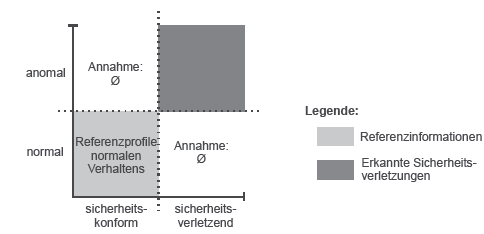
\includegraphics[width=0.45\textwidth]{aa4.png}
	\caption{Klassifikationsebenen der lern- bzw. messbasierten Anomalieerkennung \cite{5}}
	\label{fig3}
\end{figure} \noindent
\textbf{Missbrauchserkennung}\\
Die Missbrauchserkennung, die auch als Signaturanalyse
bezeichnet wird, sucht die Analysekomponenten nach konkreten Sicherheitsverletzungen ab. Dazu verwendet sie vorher definierte Angriffsmuster, welche als Signaturen bezeichnet werden. Während der Analyse werden die Audit-Daten dann auf Übereinstimmung mit den definierten
Signaturen untersucht und die Übereinstimmungen als Sicherheitsverletzung
angezeigt. Ein Nachteil hierbei ist das für die Erkennung eines Angriffs eine entsprechende Signatur vorliegen muss. Dementsprechend können mit diesem Ansatz nur bereits bekannte Angriffsarten erkannt werden.\\
\begin{figure}
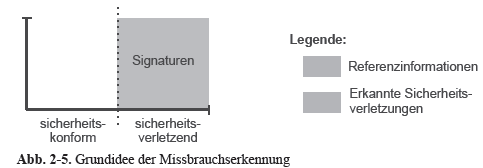
\includegraphics[width=0.45\textwidth]{aa5.png}
	\caption{Grundidee der spezifikationsbasierten Anomalieerkennung \cite{5}}
	\label{fig4}
\end{figure} \noindent
\subsubsection{Reaktionskomponenten}
\label{sec:reaction}
Nachdem etwaige Sicherheitsverletzungen durch die Analysekomponenten erkannt
wurden, werden die Reaktionskomponenten des Intrusion Detection Systems veranlasst entsprechende
Reaktionen durchzuführen. Es wird grundlegend zwischen passiven
und aktiven Reaktionen unterschieden. Passive Reaktionen liefern lediglich Informationen
an den Nutzer des IDS und überlassen diesem dann die Ergreifung
weiterer Maßnahmen. Aktive Reaktionen umfassen aber das automatische oder
halbautomatische Auslösen von Aktionen. Hierbei sind zum Beispiel gezielte Aktionen gegen den Angreifer wie das Blockieren von Netzwerkdiensten, die Benachrichtigung umgebender Systeme oder die Sammlung zusätzlicher Informationen möglich. \cite{5}

\subsection{Network-based IDS}
\label{sec:nw-based IDS}
Network-based IDS (NIDS) sind spezielle IDS die versuchen, den Paketverkehr im Netzwerk aufzuzeichnen, zu analysieren und verdächtige Aktivitäten zu melden. Sie versuchen also aus dem Netzwerkverkehr Angriffsmuster zu erkennen.\\
Netzwerkbasierte IDS überwachen in Echtzeit folgende Aktivitäten:
\begin{itemize}

\item Auslastung des Netzwerks
\item Kommunikationsbeziehungen
\item Überwachung bestimmter Ports\\
\end{itemize}
Die Erkennung von Attacken basiert dabei auf zwei Analyseverfahren:
\begin{itemize}
\item Erkennung von Abweichungen im normalen Netzwerkverkehr
\item Erkennung nach Mustern (Signaturen) für Einbrüche\\
\end{itemize}
Hier werden auch gleichzeitig die Schwachstellen von netzwerkbasierten IDS erkennbar:
\begin{itemize}
\item Definition „normaler Netzwerkverkehr“
\item Auswertung der Logfiles
\item Positionierung der IDS/IPS Lösung im Netzwerk
\item Aktualität und Verlässlichkeit der Signaturen
\item Sichere Verbindung IDS/IPS zum Log-Server
\item Absicherung des Log-Servers
\end{itemize}
\cite{8}

\subsection{Host-based IDS}
\label{sec:host based IDS}
Host-based IDS (HIDS) gehören zu den ältesten Arten von Angrifferkennungssystemen. Ursprünglich wurden sie zu militärischen Zwecken entwickelt und sollten die Sicherheit von Großrechnern garantieren. Voraussetzung ist dass ein HIDS auf jedem zu überwachendem System installierten sein muss. Der Begriff \grqq{}Host\grqq{} bezieht sich hier auf jedes System auf dem ein solches Host-based IDS installiert ist. Das HIDS muss das Betriebssystem des Hosts unterstützen.
Das HIDS bezieht seine Informationen aus Kernel-Daten, Log-Dateien und anderen Systemdaten wie zum Beispiel einer Registrierungsdatenbank.\\\\\\

Es erhält seine Informationen aus Log-Dateien, Kernel-Daten und anderen Systemdaten wie etwa der Registrierungsdatenbank. Sobald in den genannten Daten ein Angriff erkannt wird, schlägt es Alarm. Als Untergruppe der HIDS bestehen noch sogenannte „System Integrity Verifiers“, die mit Prüfsummen bestimmen ob Veränderungen am System vorgenommen wurden.\\

Vorteile:
\begin{itemize}
\item Sehr spezifische Aussagen über den Angriff.
\item Kann ein System umfassend überwachen.
\end{itemize}
Nachteile:
\begin{itemize}
\item Kann durch einen DoS-Angriff ausgehebelt werden.
\item Wenn das System außer Gefecht gesetzt wurde, ist auch das IDS lahmgelegt. 
\end{itemize}
\cite{8}

\subsection{Rechtliche Aspekte im Umgang mit IDS}
\label{sec:law ids}
\grqq{}\textit{Im Rahmen ihres Einsatzes zur Erkennung von Angriffen und Sicherheitsverletzungen zeichnen IDS eine Vielzahl von Daten auf. Diese Daten sind teilweise personenbezogen bzw. lassen die Zuordnung von Personen zu bestimmten Aktivitäten zu. Beispiele hierfür sind}
\begin{itemize}
\item \textit{die Aufzeichnung unberechtigter Zugriffsversuche auf Daten,}
\item \textit{die Aufzeichnung unberechtigter Zugangsversuche zu Anwendungen,}
\item \textit{die Aufzeichnung der IP-Adressen oder Domain-/Rechnernamen, von denen aus Angriffe oder Angriffsversuche gestartet wurden.}\\
\end{itemize}
\textit{Ein Grund des Einsatzes von IDS kann gerade darin bestehen, Angriffe zurückzuverfolgen und ihre Verursacher ermitteln zu können. Ob und welche personenbezogenen Daten aufgezeichnet werden, hängt dabei stark von der Einsatzweise und Konfiguration bzw. Kalibrierung des IDS ab. Dies soll an den folgenden zwei Einsatzbeispielen verdeutlicht werden:}
\begin{itemize}
\item \textit{Einsatz des IDS zum ergänzenden Schutz des Internet-Übergangs}\\

\textit{Beim Einsatz eines IDS als ergänzende Maßnahme zum Schutz des Internet-Übergangs, wie er im Vordergrund des Leitfadens steht, fallen typischerweise kaum personenbezogene Daten an. Für von außen initiierte Angriffe liegen im Allgemeinen lediglich IP-Adressen (als Pseudonyme) vor. Um einen Personenbezug herzustellen, ist sowohl die Auflösung der IP-Adresse durch den zugehörigen DNS-Namen erforderlich als auch die Ansprache des Unternehmens bzw. der Organisation, der dieser Name zugeordnet ist. Häufig ist diese Zuordnung aufgrund lediglich temporär zugeordneter oder gefälschter IP-Adressen nicht möglich. Interne Personenbezüge ergeben sich insbesondere, falls das IDS auch dazu eingesetzt wird, die IT-Systeme am Internet-Übergang vor unberechtigten Zugriffen aus dem internen Netz zu überwachen. In diesem Fall werden typischerweise Login-Namen oder IP-Adressen (als Pseudonyme) aufgezeichnet.}
\item \textit{Einsatz des IDS zur Überwachung des internen Netzes}\\

\textit{Eine weitergehende interne Überwachung verbunden mit einem höheren Aufkommen an personenbezogenen Daten ist gegeben, wenn IDS-Sensoren im internen Netz eingesetzt werden. Diese Einsatzweise kann z. B. dazu dienen, Angriffe und Sicherheitsverletzungen, die von Innentätern initiiert werden, oder Verstöße gegen interne Richtlinien zu erkennen.}\\
\end{itemize}
\textbf{\textit{Relevante gesetzliche Vorgaben}}
\textit{Bei der datenschutzrechtlichen Einstufung der gesamten vom IDS aufgezeichneten Daten über erkannte Ereignisse sind folgende bundesdeutsche Gesetze zu beachten: Die Beschreibung erhebt keinen Anspruch auf Vollständigkeit. Zudem wurde EU-Recht im Rahmen der Ausarbeitung nicht berücksichtigt.}\\
\begin{itemize}
\item \textit{Das Bundesdatenschutzgesetz (BDSG, Stand 19.7.2002), §§3a, 4, 4a, 5, 11, 14, 19a, 28 und 31.}
\item \textit{Die Telekommunikations-Datenschutzverordnung (TDSV, Stand 21.12.2000), §3.}
\item \textit{Das Gesetz über den Datenschutz bei Telediensten (TDDSG, Stand 14.12.2001), §§4-6.}
\item \textit{Das Gesetz über die Nutzung von Telediensten (TDG, Stand 14.12.2001), §4.}
\item \textit{Das Betriebsverfassungsgesetz (BetrVG, Stand 10.12.2001), §§87 und 90 für nicht-öffentliche oder öffentlich-rechtliche Wettbewerbsunternehmen.}
\item \textit{Das Personalvertretungsgesetz des Bundes (BPersVG, Stand 9.7.2001) bzw. des zuständigen Landes, hier beispielhaft §75 BPersVG.}\grqq{}
\end{itemize}
\cite{9}\\\\
\grqq{}\textit{Die gesammelten Auditdaten stellen nach §416 der Zivilprozessordnung kein rechtsverbindliches Beweismittel dar, wie z. B. ein notariell beglaubigtes Schriftstück. Die Daten unterliegen der freien Beweisführung, womit sie den gleichen gerichtlichen Status wie eine Zeugenaussage haben und ihre Beurteilung im Ermessen des Gerichtes liegt. Der Grund für die Einordnung als nicht rechtsverbindliches Beweismittels gründet sich auf die Tatsache, dass die Auditdaten nachträglich modifiziert werden können und somit als nicht manipulationssicher gelten. Um den Beweiswert zu erhöhen, sollten die Auditdaten vertrauenswürdig sein, es bedarf also der Sicherstellung der Integrität (z. B. durch eine digitalen Signierung der gesammelten Daten durch das IDS). Die dazu verwendeten Maßnahmen sollten aber ebenfalls vor Gericht nachgewiesen werden können (z. B. die Geheimhaltung des privaten Schlüssels, Vertrauenswürdigkeit).}\grqq{}
\cite{6}

\section{Honey Pot Systeme}
\label{sec:honey pot systems}
Ein Honigtopf oder englisch honeypot ist eine Einrichtung, einen einen Angreifer vom eigentlichen Ziel ablenken soll und ihn in einen Bereich hineinziehen soll, der ihn sonst nicht interessiert hätte. Der Name stammt aus der Natur wo man Bären oft mit einem Honigtopf oder ablenken oder sogar in die Falle locken kann.
Ein Honeypot ist also konkret ein Server der bestimmte Netzwerkdienste eines Rechnernetzes oder einfach das Verhalten eines Users simuliert. Honeypots werden vorrangig dazu eingesetzt, um Informationen über das Angriffsmuster und das Angreiferverhalten zu erhalten. Erfolgt durch den Angreifer ein Zugriff auf so einen Honey Pot, werden alle damit verbundenen Aktionen protokolliert und ggf. ein Alarm ausgelöst. Das wirklich wichtige reale Netzwerk bleibt vom Angriff möglichst verschont, da es besser gesichert ist als der Honeypot.\\

Die Idee hinter dem Einsatz von Honeypot-Systemen ist in einem Netzwerk einen oder am besten mehrere Honeypots zu installieren, die keine vom Anwender oder anderen Kommunikationspartnern benötigten Dienste bieten und so im Normalfall niemals angesprochen werden. Ein Angreifer der jetzt aber nicht zwischen einem realen Server und einem Honeypot unterscheiden kann und routinemäßig das Netz auf Schwachstellen untersucht wird natürlich den schlechter gesicherten Honeypot als Angriffsziel bevorzugen. Der Zugriff wird protokolliert und da ein Honeypot ein ungenutztes System ist, wird jeder Zugriff darauf als potenzieller Angriff gewertet.\\

Zudem gibt es Honeypots die Anwender simulieren (Honeyclients). Diese nutzen normale Webbrowser etc. und Angriffe auf den Browser oder Browser-Plug-Ins zu erkennen. Mehrere   Honeypots bilden ein zusammengeschlossenes Netz (Honeynet).
Ein physischer Honeypot stellt einen realen Rechner im Netzwerk mit eigener Netzwerkadresse dar. Ein virtueller Honeypot, jedoch, ist ein logisch eigenständiges System, welches durch einen anderen Rechner simuliert wird. \cite{10} \cite{11}

\section{Application Firewall}
\label{sec:application firewall}
Eine Application Firewall ist eine spezielle Art einer Firewall die input, output und/oder Zugriff zu oder von einer Applikation oder eines Dienstes kontrolliert. Eine Application Firewall arbeitet indem sie den input, output oder Zugriffe auf Systemdienste protokolliert und diese gegebenenfalls blockiert falls ein Verstoß gegen die Firewall-Policy vorliegt. Die Firewall ist dafür ausgerichtet den ganzen Netzwerkverkehr (bis zum application layer) zu kontrollieren. (Im Gegensatz zu einer stateful network firewall die ohne zusätzliche Software keinen Netzwerkverkehr einer bestimmten application kontrollieren kann)
Es werden zwei primäre Kategorien von Application Firewalls unterschieden:
\begin{itemize}
\item Network-based Application Firewalls
\item Host-based Application Firewalls
\end{itemize}

\subsection{Host-based Application Firewall}
\label{sec:host-based application firewall}
Eine host-based Application Firewall ist in der Lage input, output und/oder Systemdienstzugriffe an oder von einer Application zu protokollieren. Das passiert durch die Analyse der Informationen eines System-calls(und/oder zusätzlich zu einem network stack). Ein wichtiges Merkmal der host-based Application Firewall ist dass sie nur eine Sichehreit für Applications die auf demselben Host laufen bieten kann.\\

Die HBAFs bestimmen ob ein Prozess eine Verbindung akzeptieren sollte oder nicht. Sie benutzen dabei socket calls um die Verbindungen zwischen dem Application layer und den unteren layers des OSI-Modells herauszufiltern. Diese Firewalls arbeiten ähnlich wie Paketfilter, jedoch geben Application Firewalls bestimmte Filterregeln (erlauben/blockieren) auf Prozessbasis vor, wobei bei Paketfiltern dies auf Portbasis passiert. Allgemein werden prompts für die Definition dieser Regeln für Prozesse benutzt. Application Firewalls arbeiten außerdem sehr oft mit Paketfiltern zusammen.\\

Application Firewalls filtern zusätzlich Verbindungen durch das Überprüfen der Prozess-IDs von Datenpaketen und den Regeln für die lokalen Prozesse die in der Datenübertragung involviert sind. Der Umfang der Filterung wird wie schon beschrieben vom definierten ruleset bestimmt. Mit einer großen Vielzahl an Zusatzsoftware können application firewalls inzwischen schon sehr komplexe rulesets haben. Ein Nachteil dieser Prozess-rulesets ist dass ihre Effektivität im Filtern von jeder möglichen Verbindung mit anderen Prozessen sehr begrenzt ist. Zudem kann so ein ruleset nicht die Modifikation eines Prozesses (z.B. durch memory corruption exploits) verhindern.
\cite{12}
\subsection{Network-based Application Firewall}
\label{sec:network-based application firewall}
Eine Network-based Application Firewall ist eine Firewall die auf dem Application layer eines Protokoll-Stacks arbeiten und wird auch Proxy-based oder reverse-Proxy Firewall genannt. NBAFs konzentrieren sich auf eine bestimmte Art von Netzwerkverkehr abhängig vom Dienst.(wie zum Beispiel eine Web Application Firewall)\\

Die Implementierung einer solchen network-based Application Firewall kann durch eine Software die einfach am Host läuft, oder durch ein eigenständiges Netzwerkgerät realisiert werden. Oft ist es einfach ein Host der verschiedene Arten von Proxy-Servern benutzt um den Netzwerkverkehr abzufangen bevor dieser an den Client oder Server weitergeht. \\
Weil eine solche Firewall auf dem Application layer arbeitet ist eine Analyse des Inhalts des Datenverkehrs durchaus möglich wodurch bestimmte Inhalte wie zum Beispiel Webseiten oder Viren geblockt werden können.
\cite{13}




\newpage
\mbox{}
\nocite{*}
\bibliographystyle{unsrt}
\bibliography{literatur}

\end{document}